% !TEX root = ../main.tex

\chapter{Publications}
\label{app:pub}

\vspace{5cm}


This chapter includes copies of the publications and talks (where available) related to this thesis.

% Funding was provided to attend ISCC'16 in Oxford by Jon Bennett, Clinton Ingrams and a Graduate School Travel Award.

% A travel fund has been awarded by the DMU Faculty of Technology for travel to Australia, Sydney for the Creativity and Cognition conference in July 2013.

% De Montfort University has granted me a full 3 year bursary covering living costs and tuition fees.

\begin{enumerate}
  \item Presentation slides for IEEE ISCC'16 in Oxford, UK (March/April 2016).
  \item Conference paper ``Creative Zombie Apocalypse: A Critique of Computer Creativity Evaluation''. Proceedings of $2^{nd}$ IEEE International Symposium of Creative Computing (2016).
  \item Presentation slides for a \ac{CAS} \ac{IOCT} talk at the Phoenix in Leicester, UK (14 Oct 2015).
  \item Journal article ``The pataphysics of creativity: developing a tool for creative search''. Routledge: Digital Creativity, Volume 24, Issue 3 (2013).
  \item Presentation slides for Creativity and Cognition conference in Sydney, Asutralia (20 June 2013).
  \item Conference paper ``Creative Search Using Pataphysics''. Proceedings of the $9^{th}$ ACM conference on Creativity and Cognition (2013).
  \item Conference paper ``A Framework for Creativity in Search Results''. Proceedings of the $3^{rd}$ International Conference on Creative Content Technologies (2011).
\end{enumerate}

\phantomsection
\addtocounter{section}{1}
\addcontentsline{toc}{section}{\protect\numberline{\thesection}IEEE ISCC 16 conference talk}
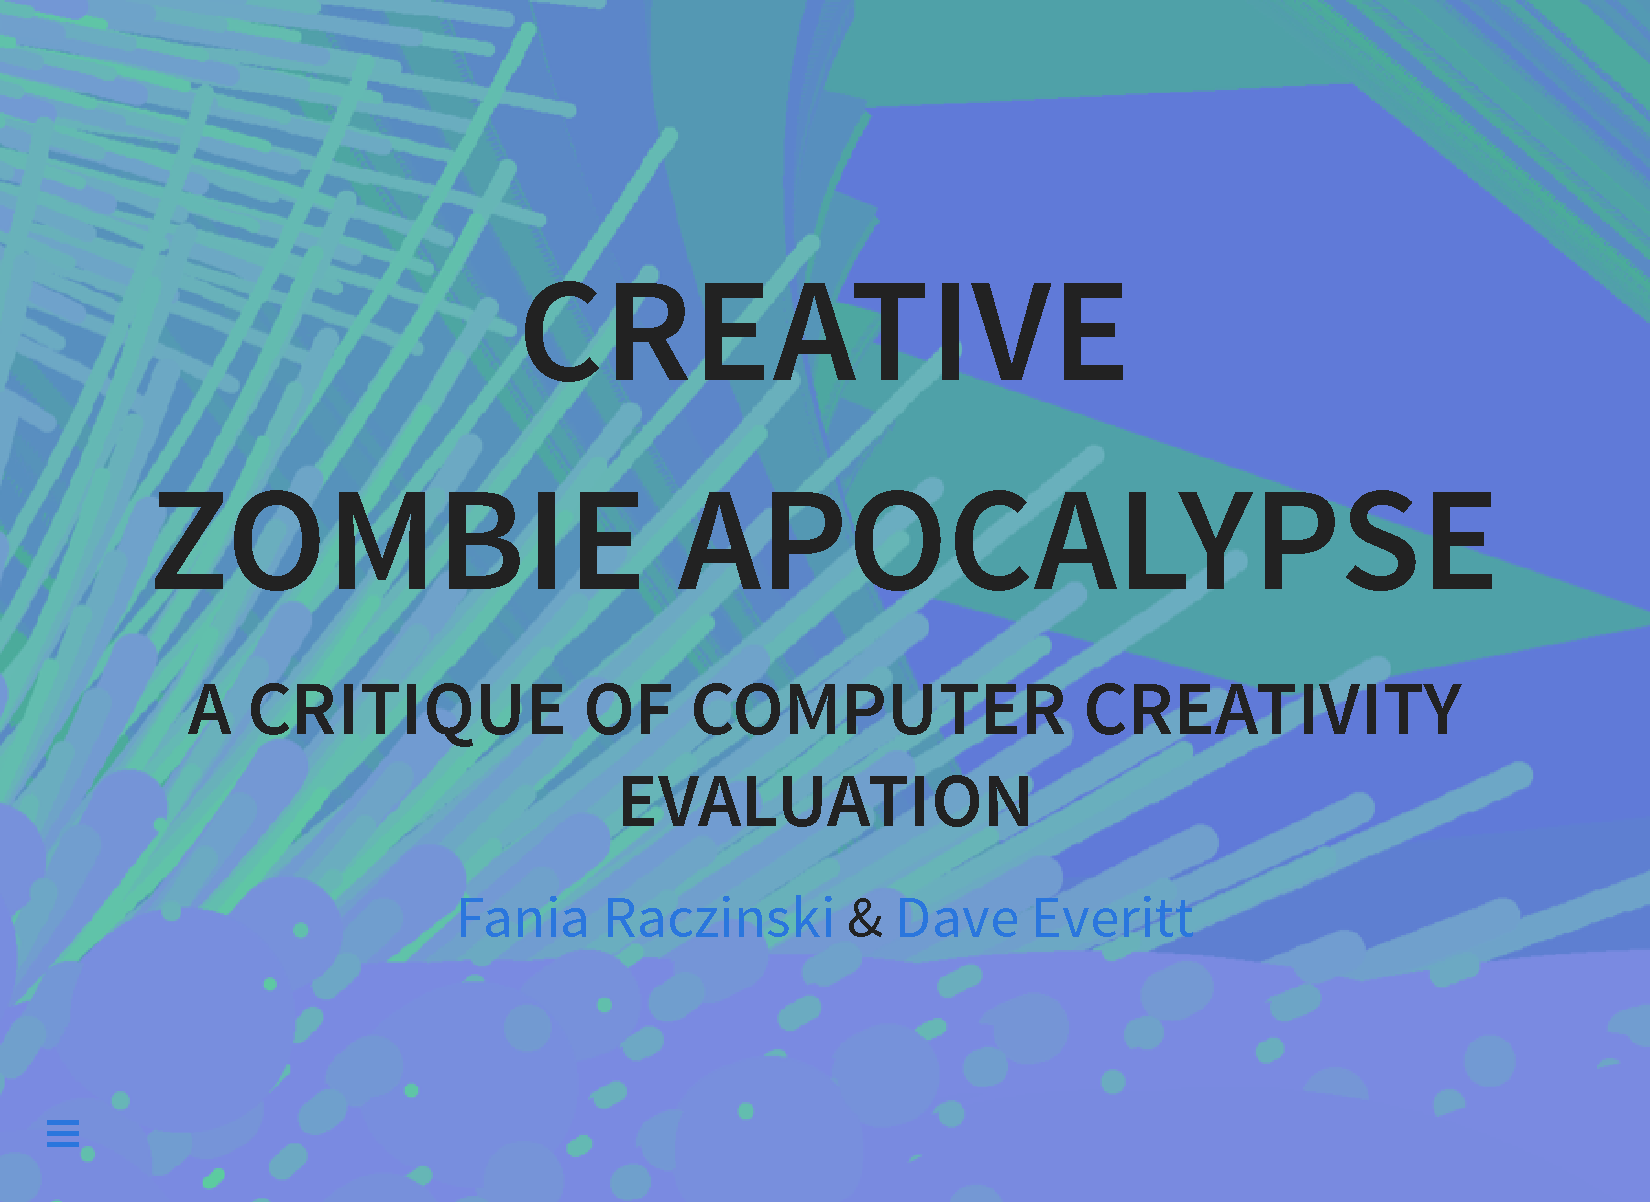
\includepdf[pages=-, nup=2x3, frame, scale=.8, pagecommand={\thispagestyle{fania}}]{RaczinskiEverittPrezi.pdf}

\phantomsection
\addtocounter{section}{1}
\addcontentsline{toc}{section}{\protect\numberline{\thesection}IEEE ISCC 16 conference paper}
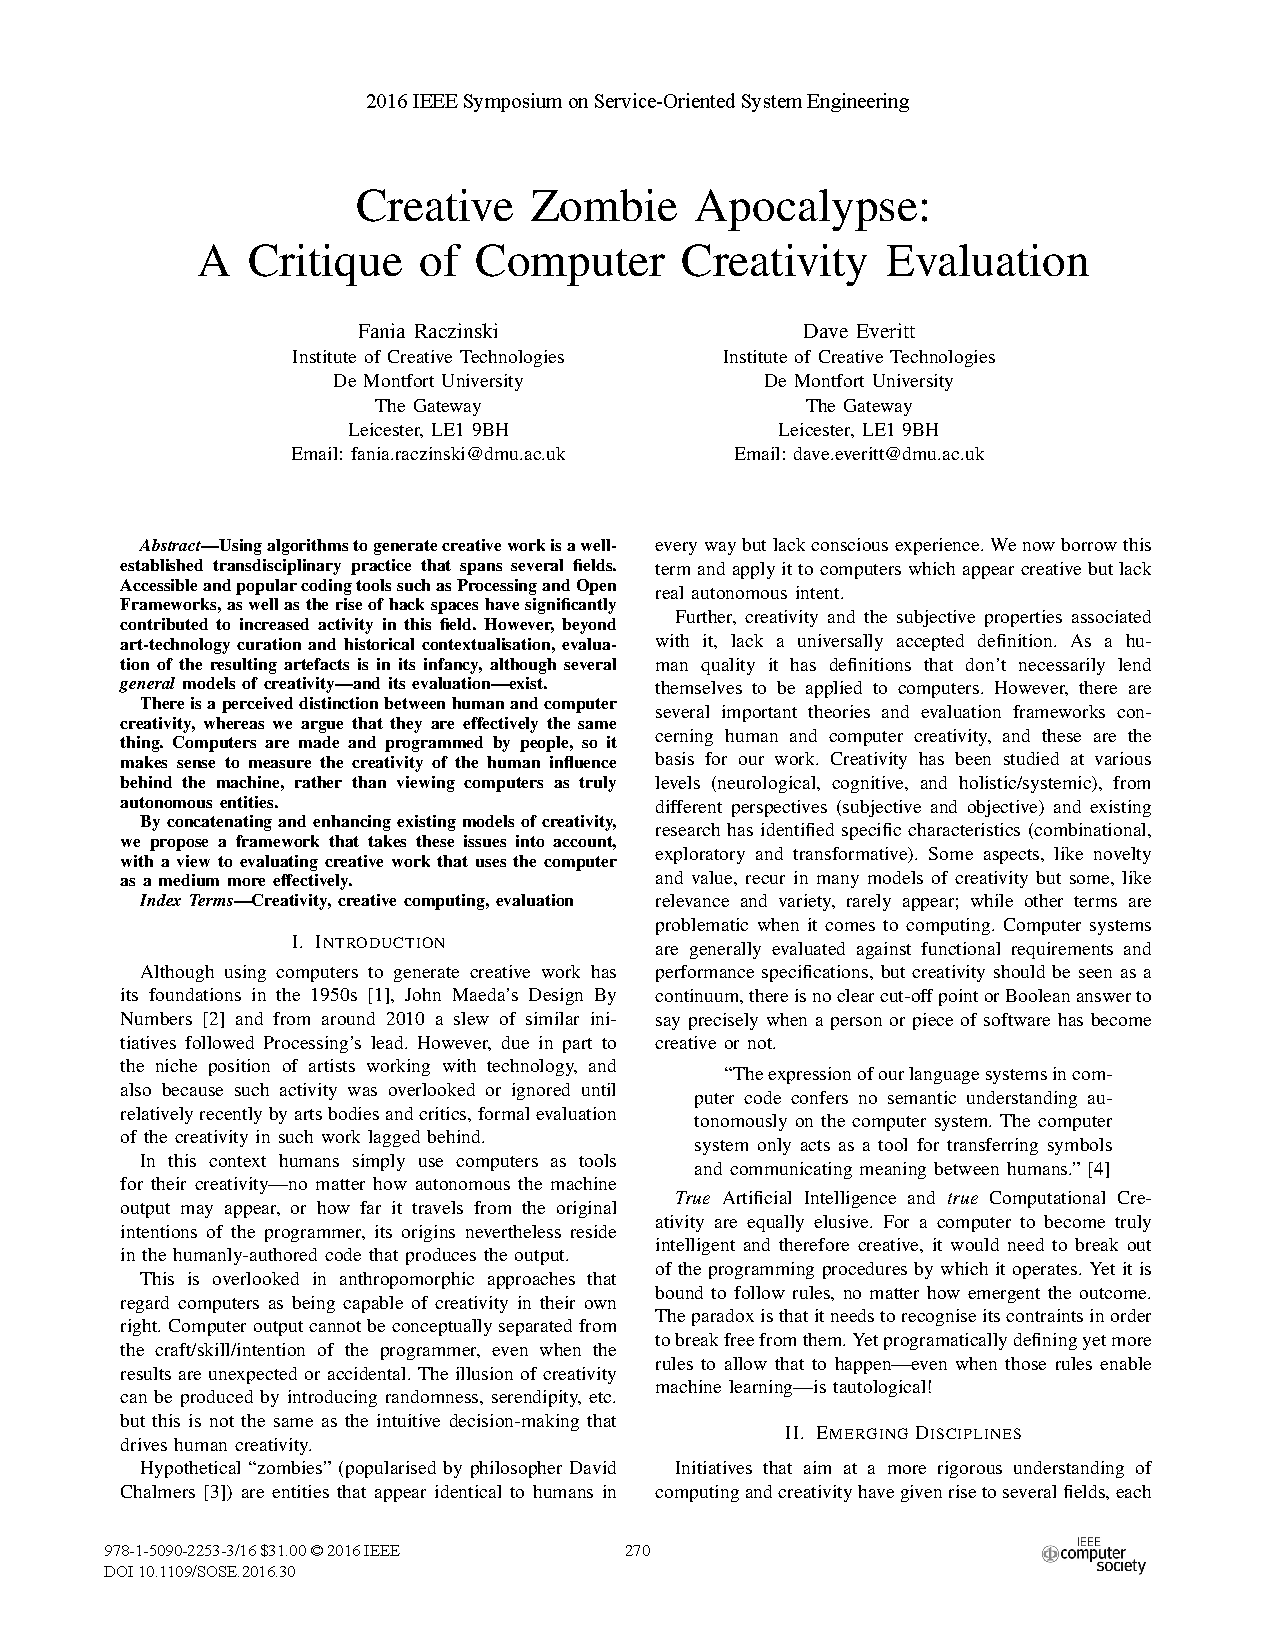
\includepdf[pages=-, frame, scale=.8, pagecommand={\thispagestyle{fania}}]{RaczinskiEveritt.pdf}

\phantomsection
\addtocounter{section}{1}
\addcontentsline{toc}{section}{\protect\numberline{\thesection}IOCT CAS talk at Phoenix}
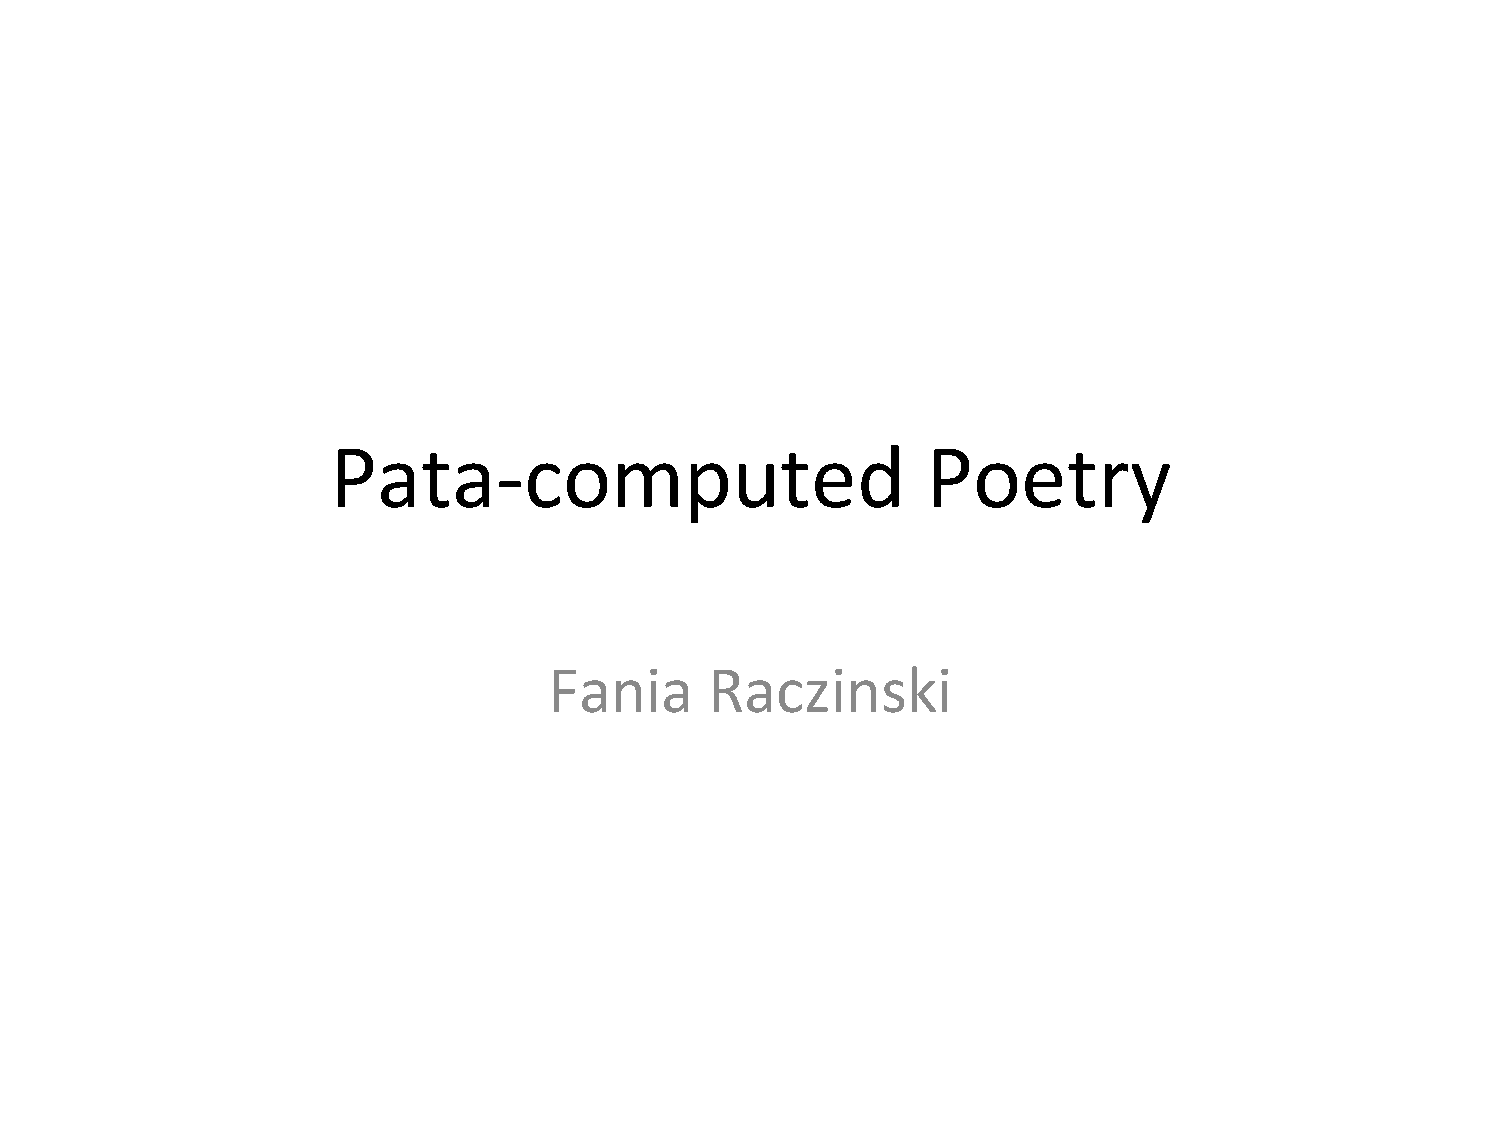
\includepdf[pages=-, nup=2x3, frame, scale=.8, pagecommand={\thispagestyle{fania}}]{CASTalk2015.pdf}

\phantomsection
\addtocounter{section}{1}
\addcontentsline{toc}{section}{\protect\numberline{\thesection}The pataphysics of creativity journal article}
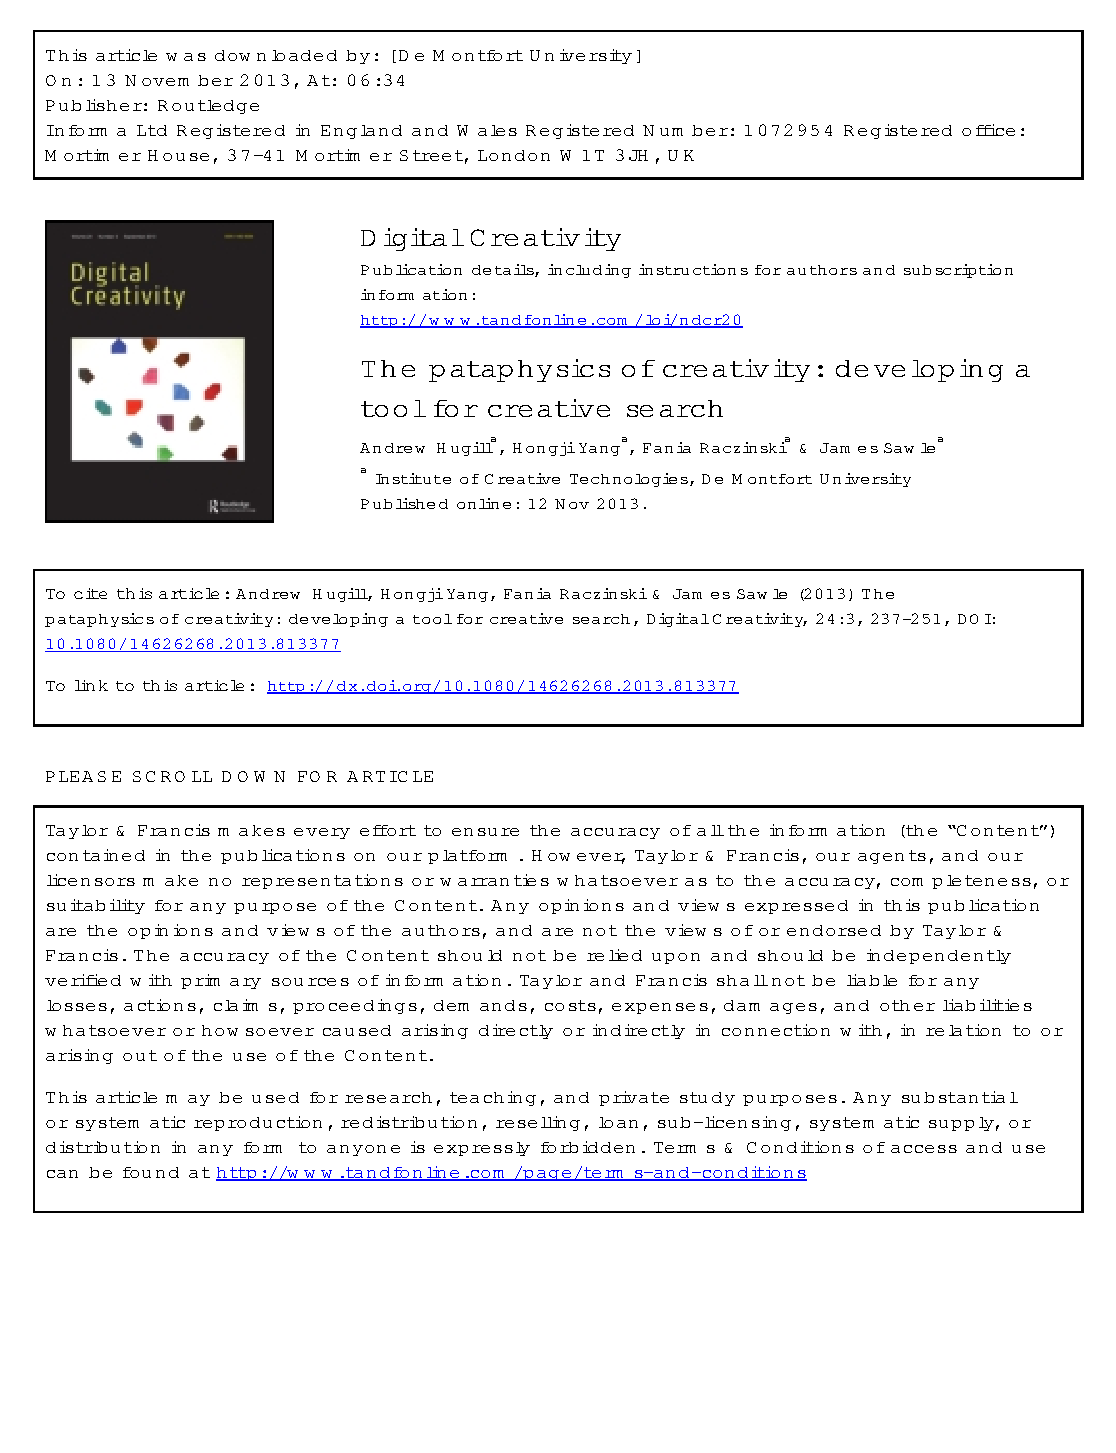
\includepdf[pages=-, frame,scale=.8, pagecommand={\thispagestyle{fania}}]{HugillYangRaczinskiSawle.pdf}

\phantomsection
\addtocounter{section}{1}
\addcontentsline{toc}{section}{\protect\numberline{\thesection}Creativity and Cognition conference talk}

\includepdf[pages=-, nup=1x3, frame,scale=.8, pagecommand={\thispagestyle{fania}}]{CC13Talk2013.pdf}

\phantomsection
\addtocounter{section}{1}
\addcontentsline{toc}{section}{\protect\numberline{\thesection}Creative Search Using Pataphysics conference paper}
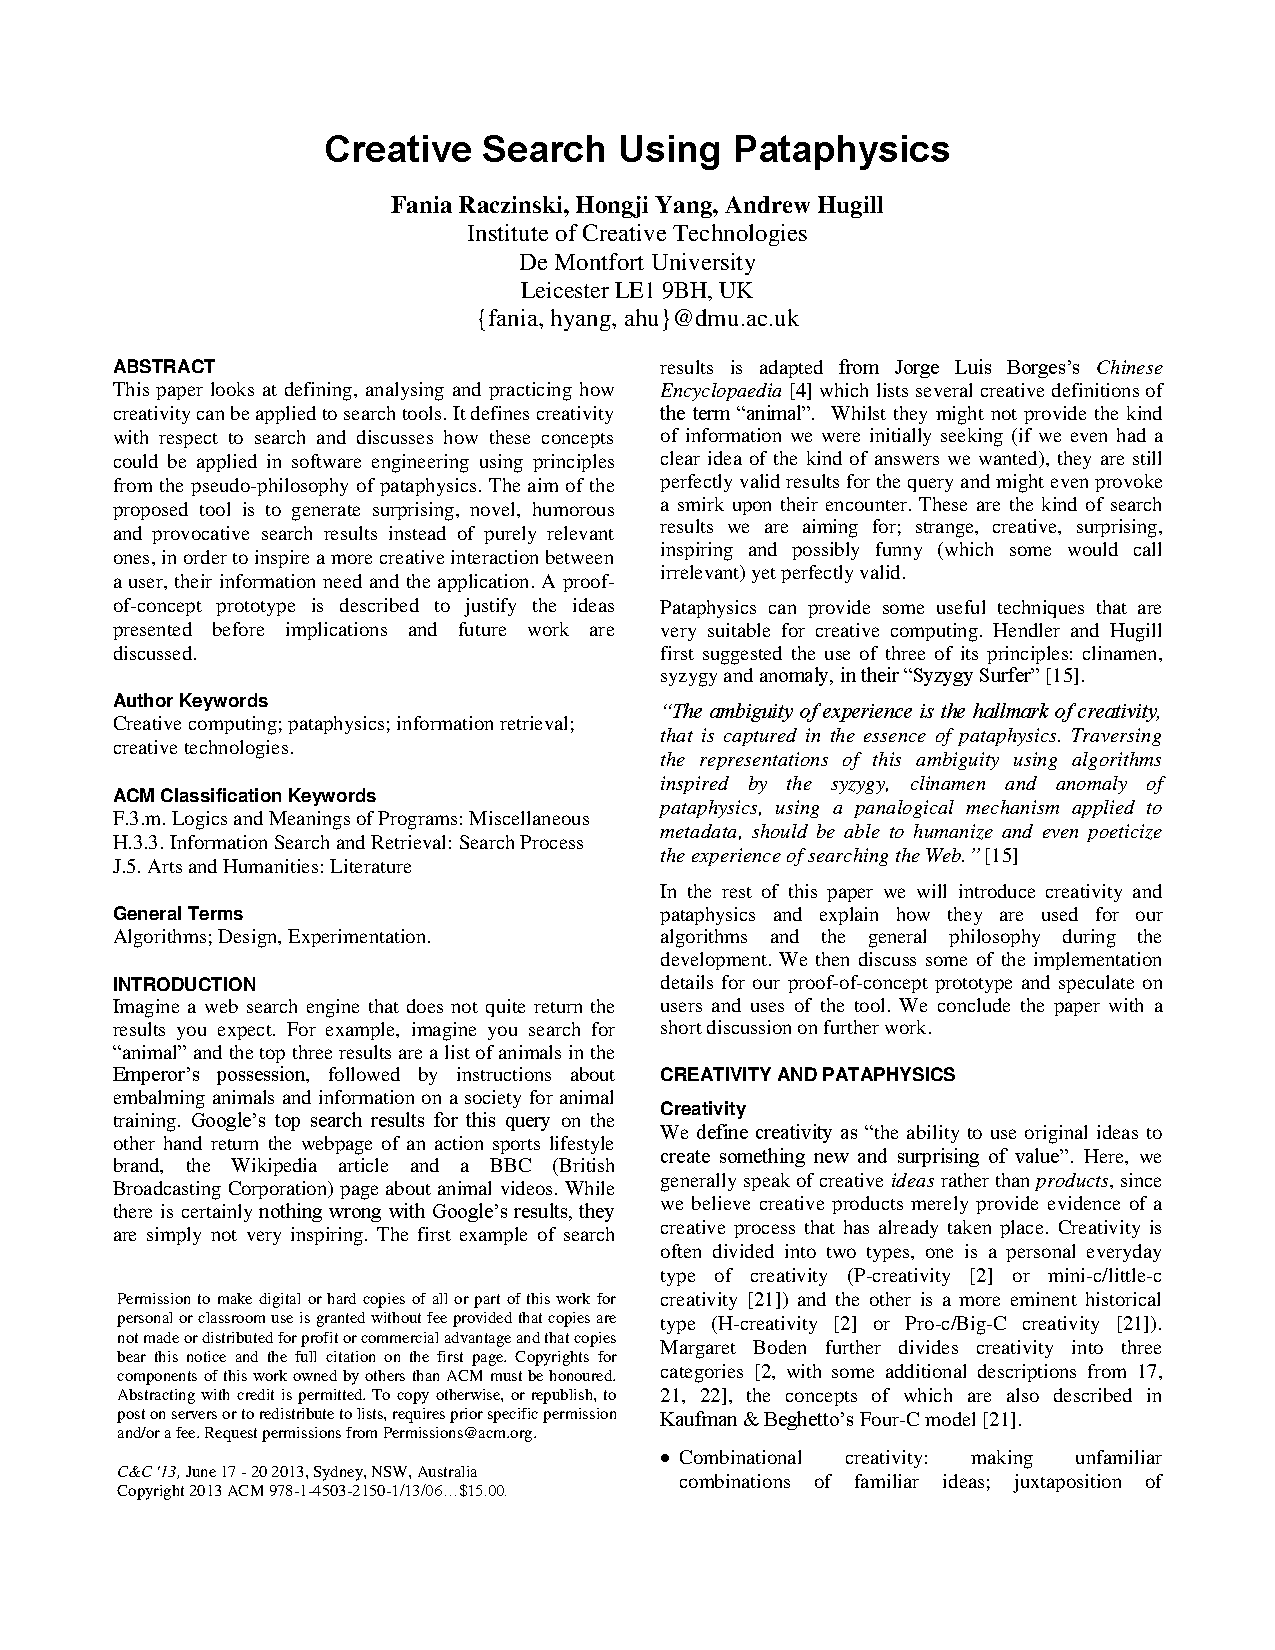
\includepdf[pages=-, frame,scale=.8, pagecommand={\thispagestyle{fania}}]{RaczinskiYangHugill.pdf}

\phantomsection
\addtocounter{section}{1}
\addcontentsline{toc}{section}{\protect\numberline{\thesection}A Framework for Creativity in Search Results conference paper}
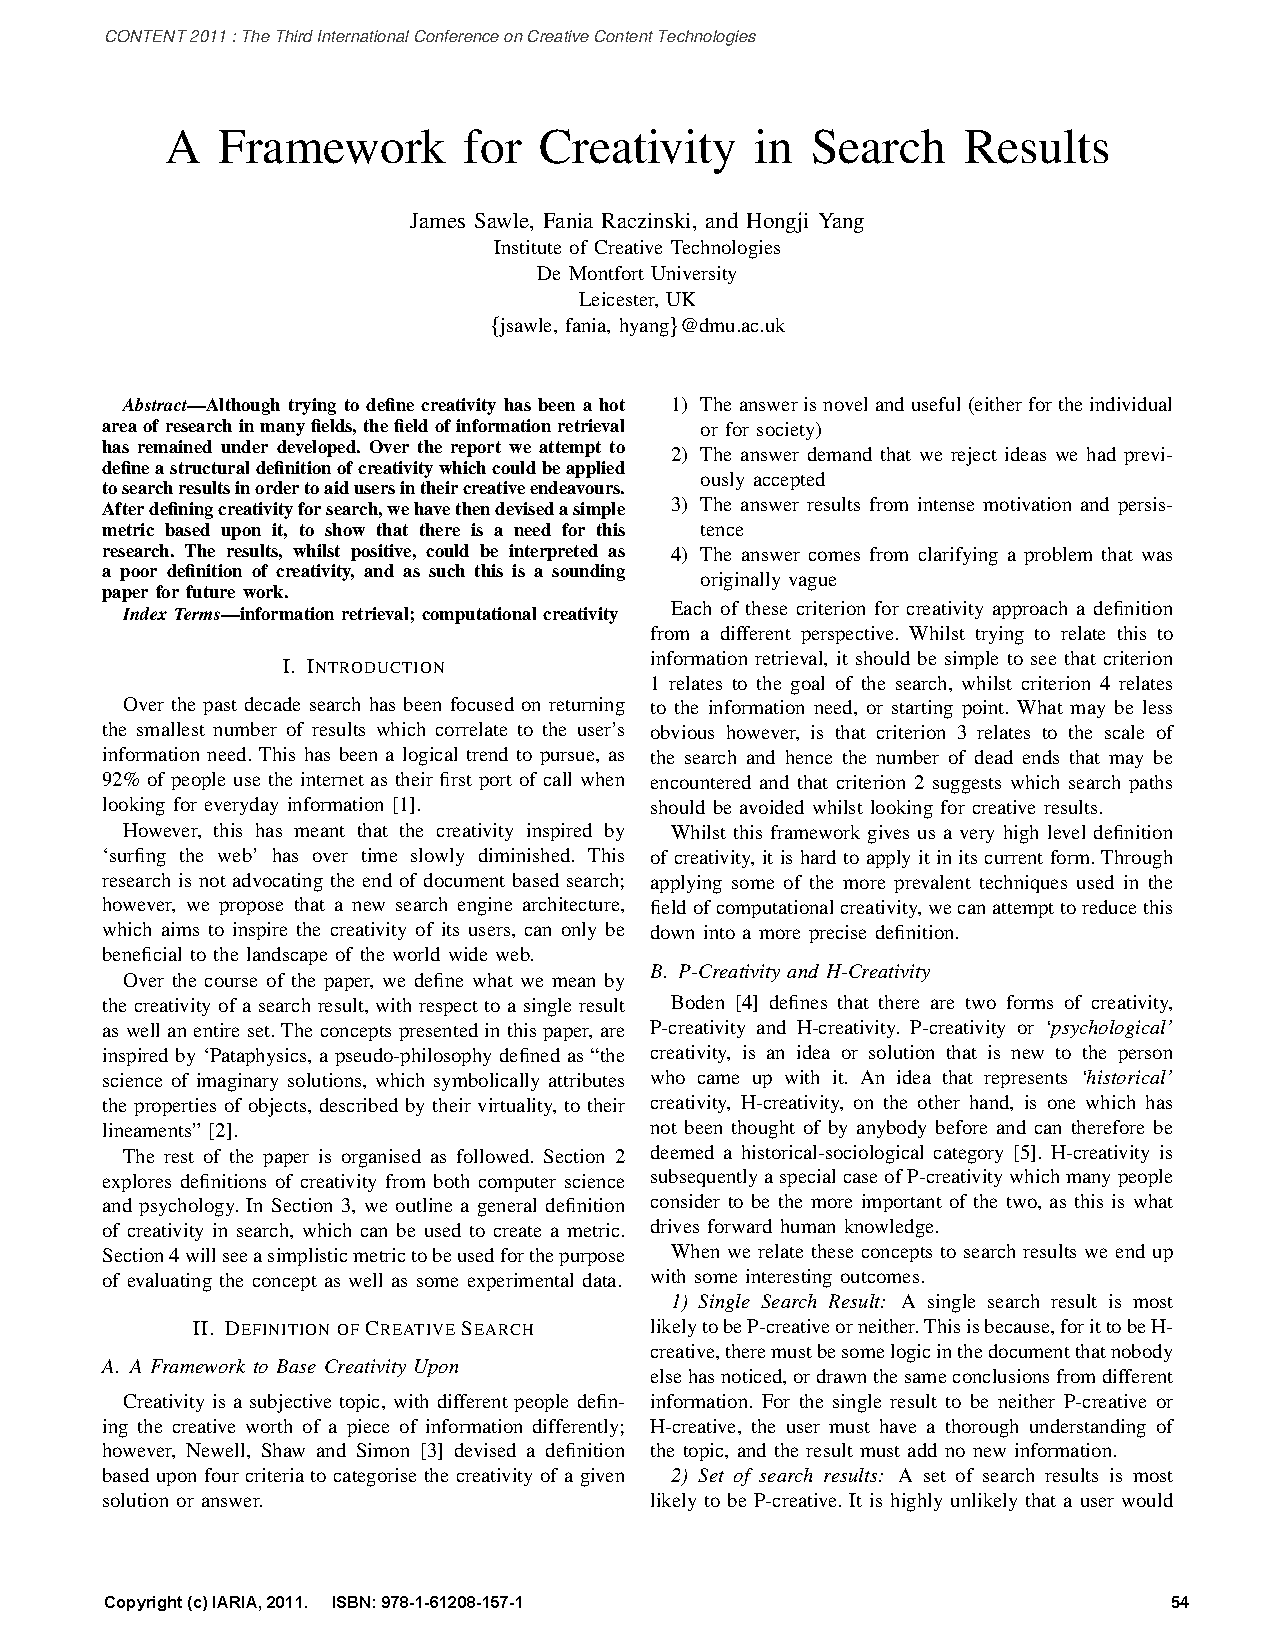
\includepdf[pages=-, frame,scale=.8, pagecommand={\thispagestyle{fania}}]{SawleRaczinskiYang.pdf}
